% TikZ代码:内存错误检测机制图
% 用于Design章节 - Cross-Framework Execution小节

\documentclass[tikz,border=10pt]{standalone}
\usepackage{tikz}
\usetikzlibrary{shapes,arrows,positioning,calc,decorations.pathmorphing}

\begin{document}

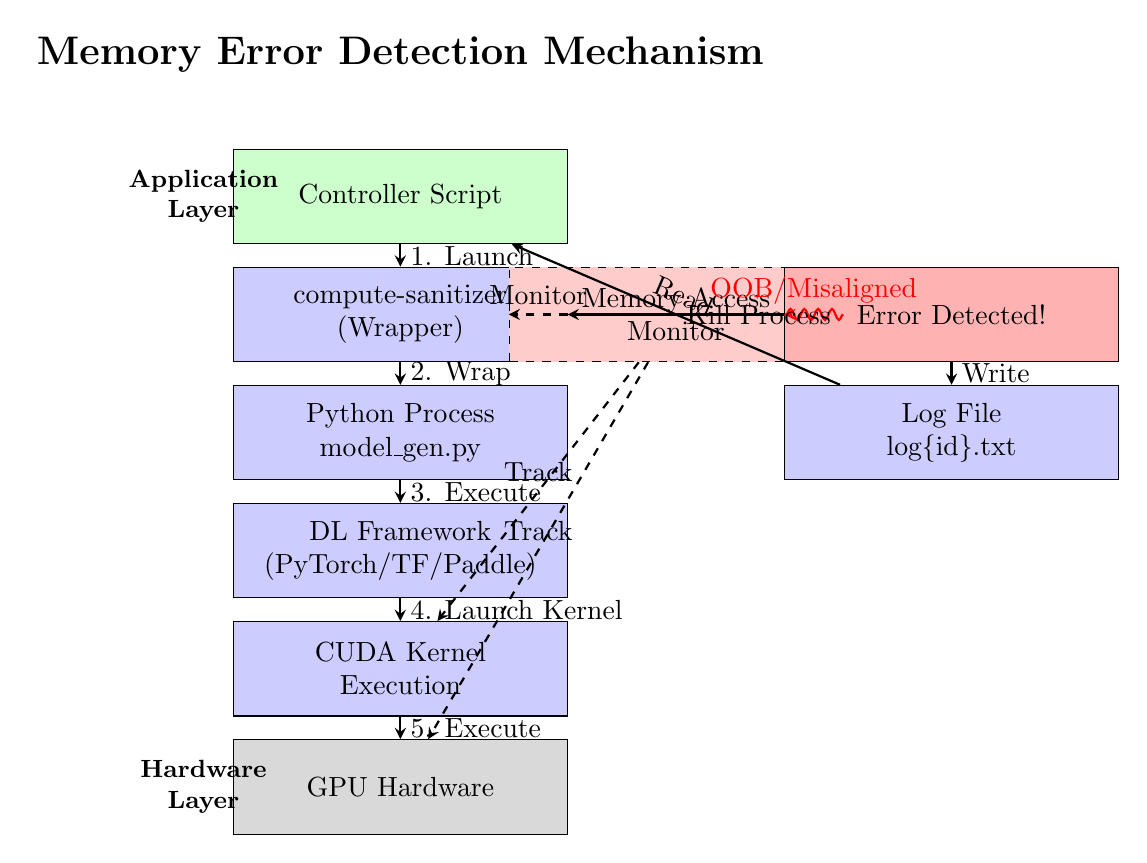
\begin{tikzpicture}[
    node distance=1.5cm,
    auto,
    layer/.style={rectangle, draw, fill=blue!20, text width=4cm, text centered, minimum height=1.2cm},
    monitor/.style={rectangle, draw, fill=red!20, text width=4cm, text centered, minimum height=1.2cm, dashed},
    arrow/.style={->, >=stealth, thick},
    error_arrow/.style={->, >=stealth, thick, red, decorate, decoration={snake, amplitude=2pt, segment length=5pt}}
]

% 应用层
\node[layer, fill=green!20] (controller) {Controller Script};
\node[layer, below of=controller] (sanitizer) {compute-sanitizer \\ (Wrapper)};
\node[layer, below of=sanitizer] (python) {Python Process \\ model\_gen.py};
\node[layer, below of=python] (framework) {DL Framework \\ (PyTorch/TF/Paddle)};
\node[layer, below of=framework] (cuda) {CUDA Kernel \\ Execution};

% 监控层
\node[monitor, right of=sanitizer, xshift=2cm] (monitor) {Memory Access \\ Monitor};

% GPU硬件
\node[layer, below of=cuda, fill=gray!30] (gpu) {GPU Hardware};

% 错误检测和日志
\node[layer, right of=monitor, xshift=2cm, fill=red!30] (error_detect) {Error Detected!};
\node[layer, below of=error_detect] (log) {Log File \\ log\{id\}.txt};

% 连接线:正常执行流程
\draw[arrow] (controller) -- node[right] {1. Launch} (sanitizer);
\draw[arrow] (sanitizer) -- node[right] {2. Wrap} (python);
\draw[arrow] (python) -- node[right] {3. Execute} (framework);
\draw[arrow] (framework) -- node[right] {4. Launch Kernel} (cuda);
\draw[arrow] (cuda) -- node[right] {5. Execute} (gpu);

% 监控连接
\draw[arrow, dashed] (sanitizer) -- node[above] {Monitor} (monitor);
\draw[arrow, dashed] (monitor) -- node[above] {Track} (cuda);
\draw[arrow, dashed] (monitor) -- node[above] {Track} (gpu);

% 错误检测
\draw[error_arrow] (monitor) -- node[above] {OOB/Misaligned} (error_detect);
\draw[arrow] (error_detect) -- node[right] {Kill Process} (sanitizer);
\draw[arrow] (error_detect) -- node[right] {Write} (log);
\draw[arrow] (log) -- node[above, sloped] {Read} (controller);

% 标注
\node[above of=controller, yshift=0.3cm, font=\Large\bfseries] {Memory Error Detection Mechanism};

\node[left of=controller, xshift=-1cm, text width=2.5cm, font=\small, align=center] {
    \textbf{Application Layer}
};

\node[left of=gpu, xshift=-1cm, text width=2.5cm, font=\small, align=center] {
    \textbf{Hardware Layer}
};

\end{tikzpicture}

\end{document}

